
\tikzstyle{block} = [rectangle, draw, 
    text width=10em, text centered, rounded corners, minimum height=10em]
\tikzstyle{intro} = [block, fill=blue!20]  
\tikzstyle{model} = [block, fill=yellow!20] 
\tikzstyle{valid} = [block, fill=black!30!green] 
\tikzstyle{optim} = [block, fill=black!50!green] 
\tikzstyle{other} = [block, fill=black!10!purple] 
\tikzstyle{sloud} = [draw, star,fill=green!20, minimum height=2em]
\tikzstyle{ar}    = [->, thick, shorten <=8pt, shorten >=8pt]
\tikzstyle{wlock} = [rectangle, draw, 
    text width=5em, text centered, minimum height=4em]


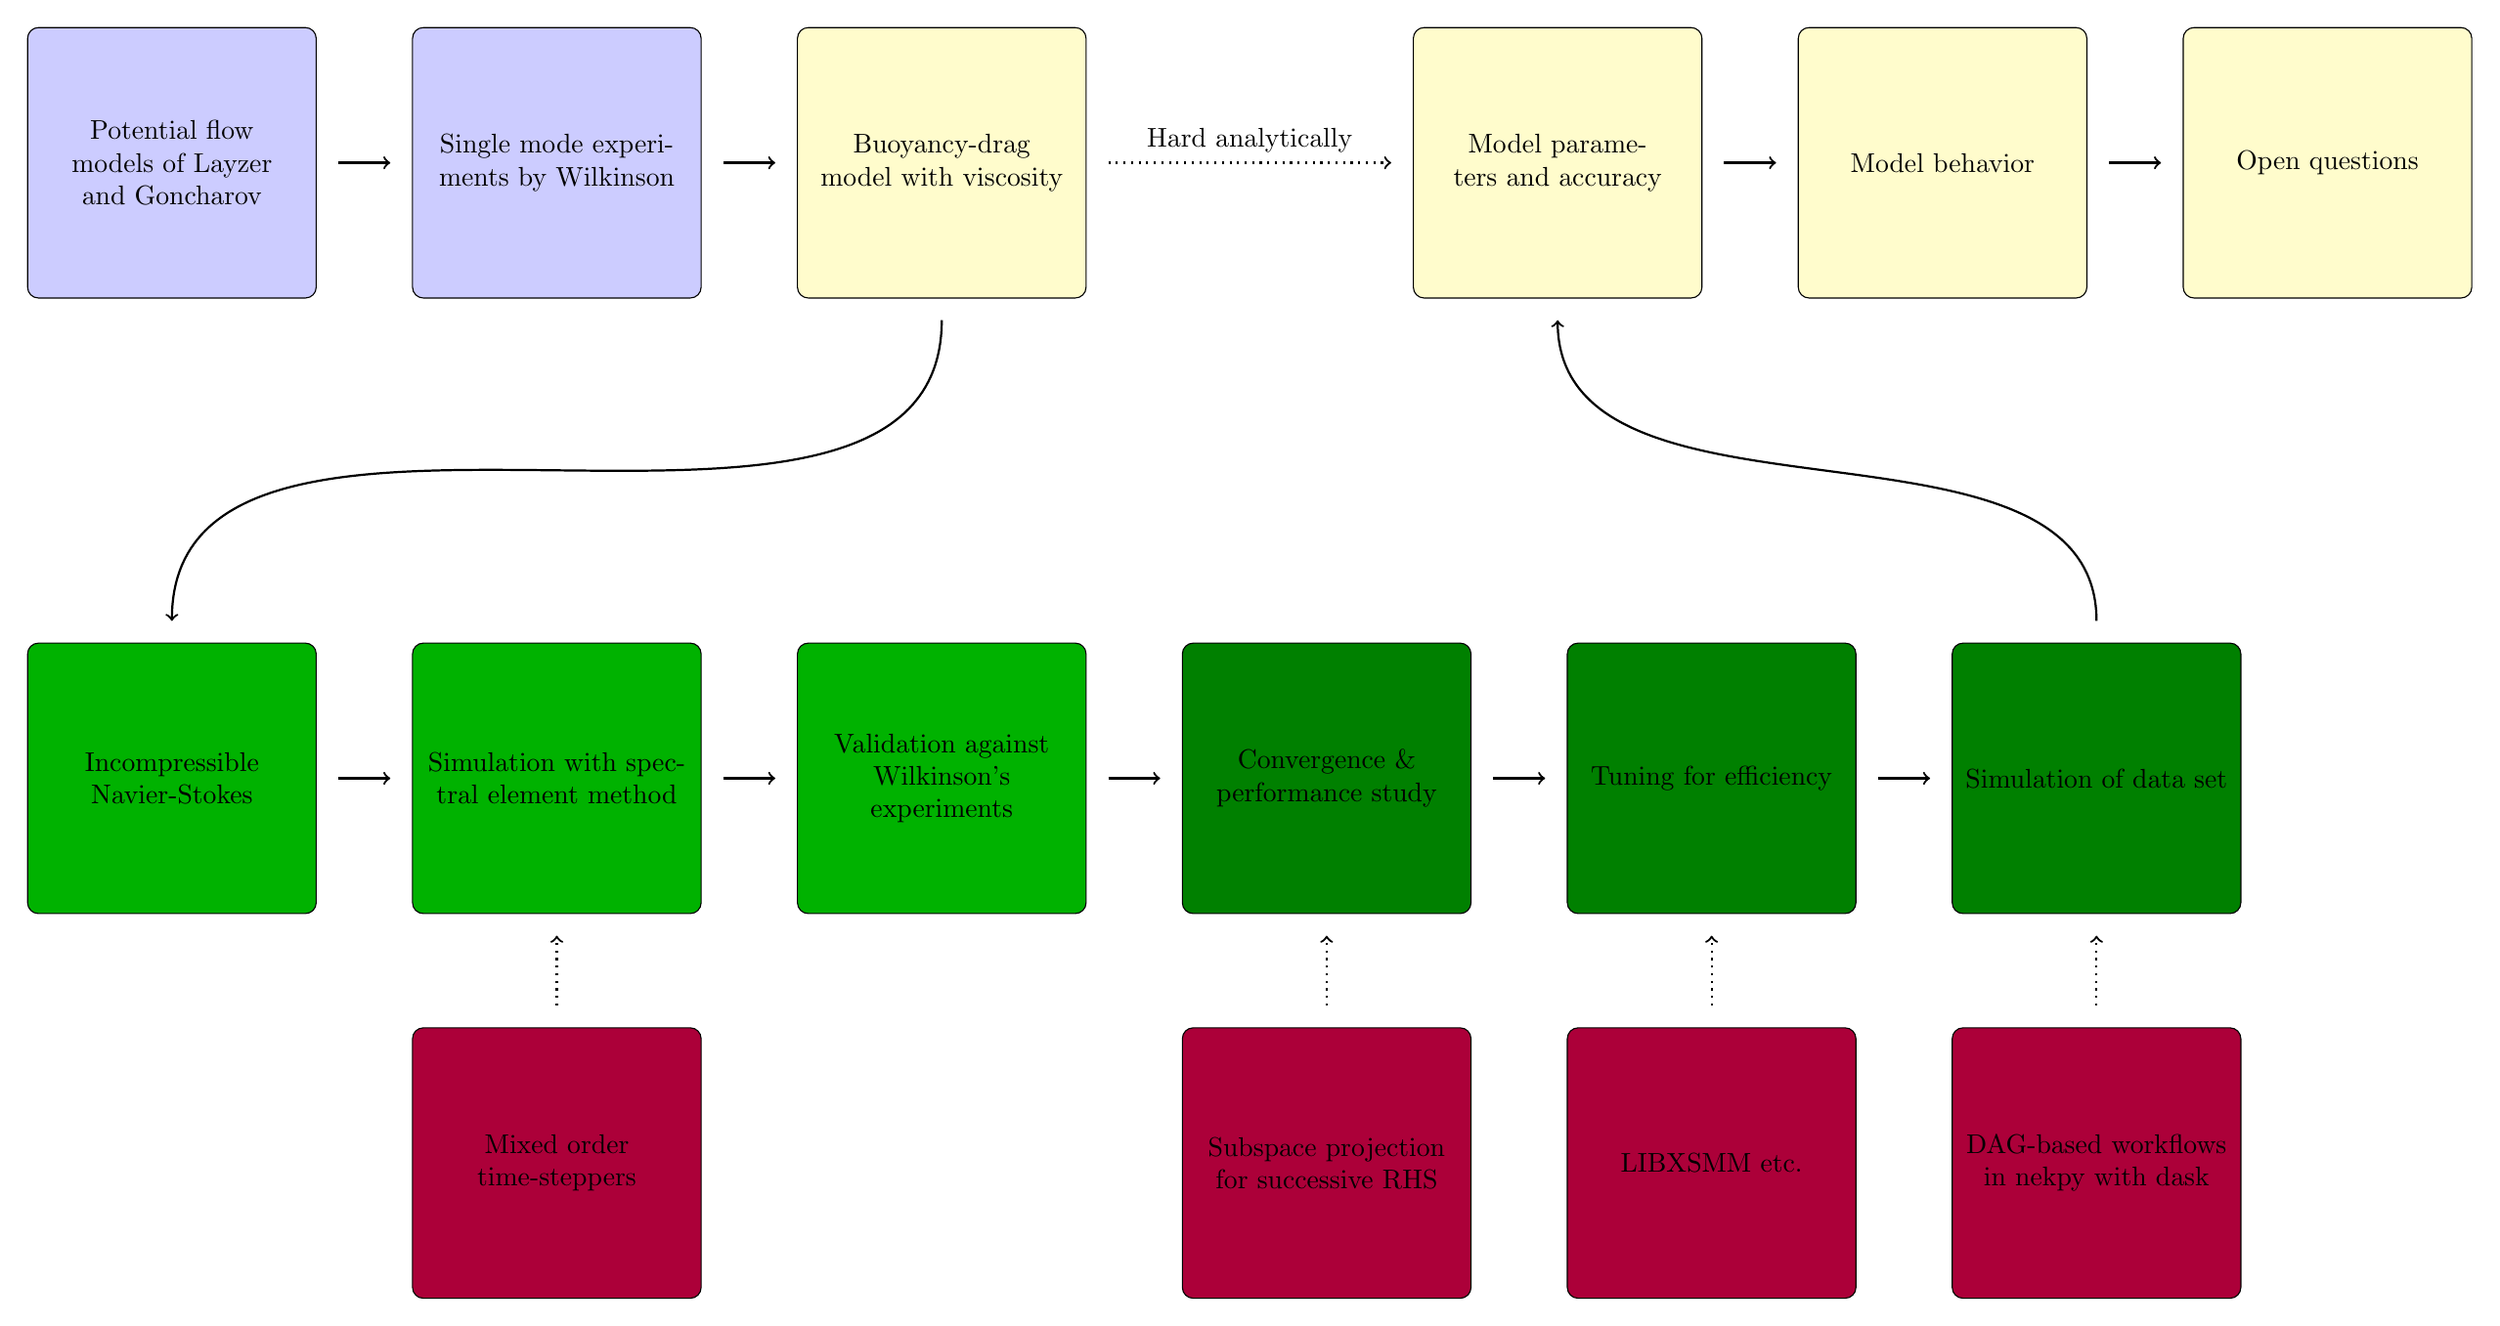
\begin{tikzpicture}[node distance=5cm, auto]
\node[intro] (layzer) {Potential flow models of Layzer and Goncharov};
\node[intro, right of=layzer] (wilk) {Single mode experiments by Wilkinson};
\node[model, right of=wilk] (bdm) {Buoyancy-drag model with viscosity};
\node[model, right of=bdm, node distance=8cm] (param) {Model parameters and accuracy};
\node[model, right of=param] (behavior) {Model behavior};
\node[model, right of=behavior] (ques) {Open questions};

\node[valid, below of=bdm, node distance=8cm] (val) {Validation against Wilkinson's experiments};
\node[valid, left of=val] (sim) {Simulation with spectral element method};
\node[valid, left of=sim] (NS) {Incompressible Navier-Stokes};
\node[optim, right of=val] (conv) {Convergence \& performance study};
\node[optim, right of=conv] (tuning) {Tuning for efficiency};
\node[optim, right of=tuning] (data) {Simulation of data set};

\node[other, below of=sim] (ts) {Mixed order time-steppers};
\node[other, below of=tuning] (xsmm) {LIBXSMM etc.};
\node[other, below of=data] (dask) {DAG-based workflows in nekpy with dask};
\node[other, below of=conv] (proj) {Subspace projection for successive RHS};

\path (layzer) edge[ar] (wilk);
\path (wilk) edge[ar] (bdm);
\path (bdm) edge[ar, dotted] node {Hard analytically} (param);
\path (param) edge[ar] (behavior);
\path (behavior) edge[ar] (ques);

\path (NS) edge[ar] (sim);
\path (sim) edge[ar] (val);
\path (val) edge[ar] (conv);
\path (conv) edge[ar] (tuning);
\path (tuning) edge[ar] (data);

\path (bdm) edge[ar, out=270, in=90] (NS);
\path (data) edge[ar, out=90, in=270] (param);

\path (ts) edge[ar, dotted] (sim);
\path (xsmm) edge[ar, dotted] (tuning);
\path (dask) edge[ar, dotted] (data);
\path (proj) edge[ar, dotted] (conv);

%\path () edge[ar] ();
%\path () edge[ar] ();

%\path (ibc) edge[ar, bend right=45] (pet);
%\path (inp) edge[ar, bend right=45] (pet);
%\path (raw) edge[ar, bend left=45] (pet);
%\path (opp) edge[ar, bend left=45] (pet);

\end{tikzpicture}
